\documentclass[20pt]{article}
\usepackage{graphicx}
\setlength\parindent{0pt}
\usepackage{amsfonts}
\usepackage{courier}
\begin{document}
\title{Soundcool's Envelope Module Specification}
\maketitle



\section*{User interface}
Following is the user interface for an envelope module in Soundcool:

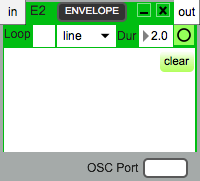
\includegraphics[scale=0.75]{gui.png} 

\begin{itemize}
    \item \textbf{Drop points:} User can drop points on the canvas by clicking. After two points are dropped, there will be lines connecting each pair of two x-adjacent points. That is, in terms of x coordinate, each pair of neighboring points. 
    \item \textbf{Drag points:} User can drag points. This will result in the connecting line also change.
    \item (Optional) \textbf{Delete points:} If possible we will implement the delete point feature, since there is none in soundcool 3.1
    \item \textbf{Clear canvas}.
    \item \textbf{Change duration:} duration indicates the time interval that the envelope on the canvas get applied to. In seconds, enter an integer greater than 1. 
    \item \textbf{Loop:} selecting loop will result in the envelope applied consecutively.
    \item The button next to duration: click to apply or bypass the current envelope. 
\end{itemize}

\newpage
\section*{Web Audio Implementation}
\subsection*{Terminology}
canvas = the window where user specifies the envelope curve\\
y-value = Y coordinate on canvas  (amplitude multiplier). Range: [0,1].\\
x-value = X coordinate on canvas (discrete sample index)\\

An envelope specification requires a JavaScript(JS) \texttt{Object} with following fields: 1) \texttt{startSample} 2) \texttt{endSample} 3) \texttt{sustainAmp} 4) \texttt{arr}. Since envelope can be looped and could be of arbitrary shape, the only way to achieve this in Web Audio is to use a Audio Buffer Source Node (ABSN). The idea is to represent user specified envelope as discrete samples in a \texttt{Float32Array}. Here is the definition of the parameters:

\subsubsection*{\texttt{startSample:(integer)\footnotemark[1] number}}
x-value where user specified curve starts\\
\subsubsection*{\texttt{endSample:(integer)\footnotemark[1] number}}
x-value where user specified curve ends; means there exists no user-selected point that has a greater x-value than \texttt{endSample}.\\
\subsubsection*{\texttt{sustainAmp:(float)\footnotemark[1] number}}
y-value where user specified curve ends\\
\subsubsection*{\texttt{arr:Float32Array} }
user specified curve stored as \texttt{Float32Array} of sample rate length (assume 44100). Note that for the samples that do not have user specified y-value, default it to 0.


\footnotetext[1]{type \texttt{number} in JS refers to both \texttt{int} and \texttt{float}. Prefix indicate whether to cast to nearest integer.}
\newpage

The figure below shows all valid envelopes and their respective outcomes. Parameters of the envelope curve are annotated as well for brevity.

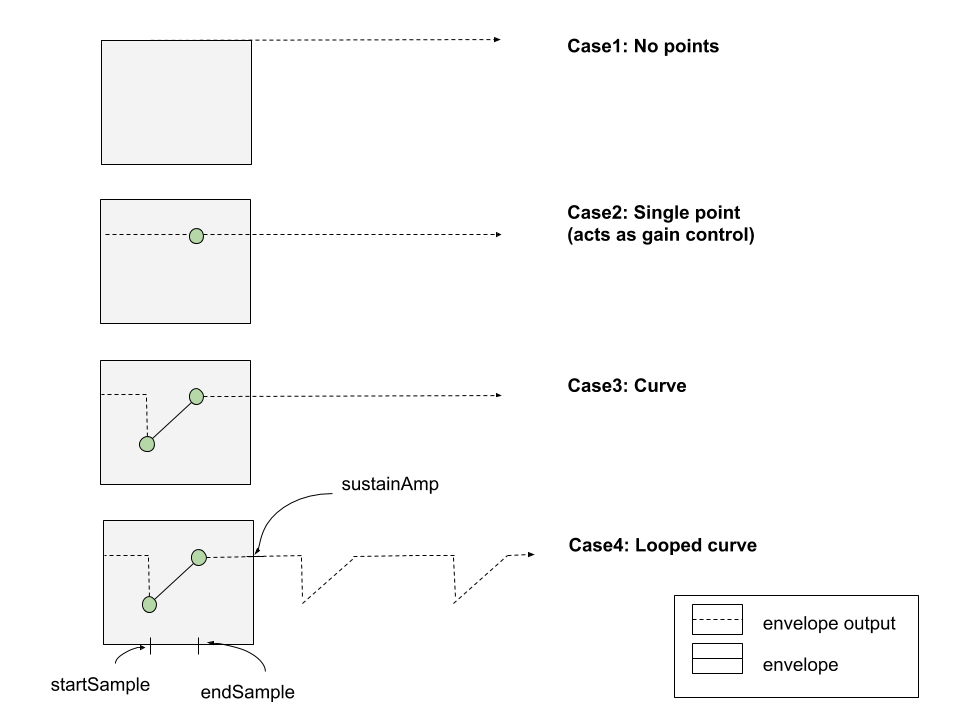
\includegraphics[width=15cm,height=12cm]{cases.png} 

Note that for the case1: set \texttt{startSample} and \texttt{endSample} to \texttt{0}. For case2: set  \texttt{startSample} = \texttt{endSample} = selected \texttt{x-value}.

\subsection*{Methods}
\subsubsection*{\texttt{set duration:number}}
\texttt{duration} is the length of wave (in seconds) to apply envelope to. \texttt{duration}  can be set by tweaking \texttt{playbackRate} audio param of ABSN.
\begin{equation}
\texttt{playbackRate = 1 / duration}
\end{equation}

\subsubsection*{\texttt{set loop:boolean}}
\texttt{loop} setter wraps ABSN's \texttt{loop} audio param.


\end{document}